\section{Resultados}

En esta seccion se analizará con experimentacion el codigo, en especial el desempeño de las dos implementaciones de máximo, antes de
evaluar se plantea como hipótesis que la implementacion concurrente de máximo va a trabajar en forma mas rápida que la otra implementación
por el hecho de que realiza mayor parte del trabajo en forma, justamente, concurrente, aprovechando más los threads disponibles.


A continuación se pasa a experimentar para corroborar esta hipótesis.

\subsection{Experimentación Tiempos}
Se realizó una experimentación que utiliza archivos generados aleatoriamente y compara los resultados de las dos funciones de máximos implementadas.\\

Las palabras se generaron utilizando el archivo $gerenador.py$ que se envía junto con el código.\\

Para la medición se corrieron 500 veces ambas funciones y se promediaron los tiempos.

\subsubsection{Tiempos de ejecucion} %diferencias entre los 2 maximos

\begin{center}
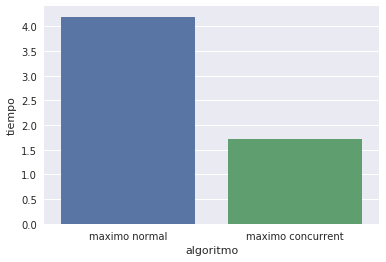
\includegraphics[width=0.8\textwidth]{imagenes/maxvsmax.png}
\end{center}

En este grafico se puede ver la comparación entre las dos implementaciones de maximo funcionando
para 5 archivos con 5 threads. Se puede ver claramente que la implementación concurrente
es más del doble de rapida.

\begin{center}
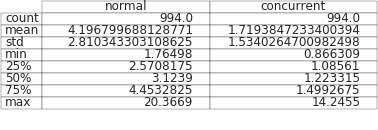
\includegraphics[width=0.8\textwidth]{imagenes/descplot.png}
\end{center}

En esta tabla se pueden ver los valores estádisticos de la comparación. Se
corrieron mil veces los algoritmos para este caso.

\begin{center}
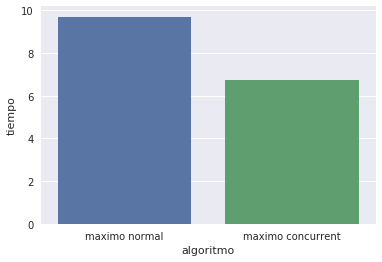
\includegraphics[width=0.8\textwidth]{imagenes/maxvsmax1thread.png}
\end{center}

Aquí se puede ver la comparación de ambos para 11 archivos con 1 solo thread.\\
Este resultado a priori es extraño ya que ambas se ejecutan de forma no concurrente. Sin embargo, al tener en cuenta que la versión no concurrente crea un hashmap para luego pasarlo a otro hashmap y ahí calcular el máximo, tiene sentido pensar que pueda haber demorado mayor cantidad de tiempo que su equivalente concurrente.

\begin{center}
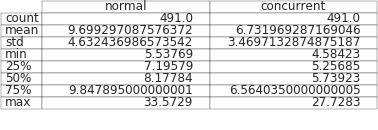
\includegraphics[width=0.8\textwidth]{imagenes/descplot2.png}
\end{center}

En esta tabla se pueden ver los valores estadísticos de la comparación, en este caso
los algorimos se corrieron 500 veces.

\subsection{Experimentación Threads}

Además, se realizó una experimentación corriendo ambas instancias variando la cantidad de threads con 1 $\leq n \geq 10$.
Ambas implementaciones se corrieron 500 veces para cada $n$ y se promediaron los tiempos arrojando los siguientes resultados:

\begin{center}
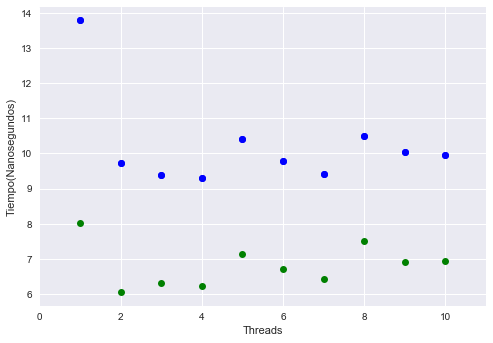
\includegraphics[width=0.8\textwidth]{imagenes/threads.png}
\end{center}

Donde el verde representa a la versión concurrente y el azul a la no concurrente.

Como esperabamos, encontramos que la versión concurrente arroja tiempos menores que su contraparte no concurrente. Sin embargo, se puede observar que al aumentar los threads no mejora los tiempos significativamente, de hecho en algunos casos los empeora. Esto podría tratarse a que al agregar palabras en la estructura se bloquean con un mutex las listas, haciendo mayores los tiempos de espera al haber muchos threads.

Por otro lado, a simple vista parece haber una correlación entre los tiempos.


